\documentclass[aspectratio=169,12pt]{beamer}
\usepackage{fontspec}
\setmainfont{CMU Serif}
\newfontfamily{\cyrillicfont}{CMU Serif}
\setsansfont{CMU Sans Serif}
\newfontfamily{\cyrillicfontsf}{CMU Sans Serif}
\setmonofont{CMU Typewriter Text}
\newfontfamily{\cyrillicfonttt}{CMU Typewriter Text}

%%% Fonts and language setup.
\usepackage{polyglossia}
%% Math
\usepackage{amsmath, amsfonts, amssymb, amsthm, mathtools} % Advanced math tools.
\usepackage{icomma} % "Умная" запятая: $0,2$ --- число, $0, 2$ --- перечисление

\usetheme{boxes}
\usecolortheme[style=light]{Nord}
\usefonttheme{Nord}
\setbeamertemplate{navigation symbols}{}%remove navigation symbols
\usepackage{minted}
\usemintedstyle{nord}

\setbeamertemplate{footline}[frame number]

%%% Polyglossia setup after  (nearly) everything as described in documentation.
\setdefaultlanguage{russian}
\setotherlanguage{english}

\usepackage{multicol}
\usepackage{xcolor}
\setlength{\columnsep}{0.5cm}

\begin{document}
\begin{frame}
   \begin{center}
    \vspace{1.5cm}
    \Large\textcolor{NordBrightBlue}{\textbf{Использование сплайнов
    третьего порядка для программной генерации некоторых заданий ЕГЭ по
    математике}}\\
        \end{center}
        \vspace{0.5cm}
        \large\textcolor{NordBlue}{\textit{Докладчик: Суматохина А.С.}}\\
        \large\textcolor{NordBlue}{\textit{Научный руководитель: Авдеев Н.Н.}}\\
        \vspace{0.5cm}
        \begin{center}
            13 апреля 2023 г.
        \end{center}
        \begin{center}
            Воронеж, ВГУ
        \end{center}
        
\end{frame}

\begin{frame}{Существующие проблемы}
    \begin{itemize}
        %TODO: Тут написан какой-то бред
        \item Дефицит заданий для подготовки
        \item Списывание ответов учениками
        \item При появлении новых заданий в экзамене — \\дефицит материалов увеличивается в разы
        \item Некоторые задания решаются слишком быстро, \\а их составление вручную занимает несоразмерно много времени.
    \end{itemize}
\end{frame}

\begin{frame}{Проект «Час ЕГЭ»}
    \large
    «Час ЕГЭ» — компьютерный образовательный проект, разрабатываемый с 2013~года при математическом факультете ВГУ в рамках «OpenSource кластера» и предназначенный для помощи учащимся старших классов подготовиться к тестовой части единого государственного экзамена.
\end{frame}

\begin{frame}{Примеры генерации задач №10}
    \begin{multicols}{2}
          
        На рисунке изображены графики функций $f (x)=a\sqrt{x}+c$ и $g (x)=kx+b$, которые пересекаются в~точках $A$ и $B$. Найдите абсциссу точки $B$.\\
        
        Ответ: $16$\\

        Решение: \\
        $f (x)=5\sqrt{x}-8$\\
        $g (x)=x-4$\\
        $A (1; -3)$\qquad
        $B (16; 12)$


        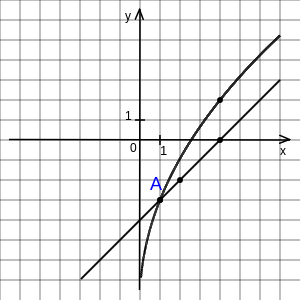
\includegraphics[width=0.4\textwidth]{images/230486231093499n0}
    \end{multicols}
         
\end{frame}

\begin{frame}{Примеры генерации задач №10}
    \begin{multicols}{2}
        На рисунке изображён график функции $f (x)=\frac{k}{x}+b$. Найдите значение $x$, при~котором $f (x)=-1,75$.\\

        Ответ: $9$\\

        Решение: \\
        $f (x)=\frac{3}{x}-2$

        
\includegraphics[width=0.4\textwidth]{images/5535657652049n0.png}
    \end{multicols}
    
\end{frame}

\begin{frame}{Примеры генерации задач №10}
    \begin{multicols}{2}
        На рисунке изображены графики функций $f (x)=\frac{a}{x+c}$ и $g (x)=kx+b$, которые пересекаются в~точках $A$ и $B$. Найдите абсциссу точки $B$.\\

        Ответ: $-16$ \\

        Решение: \\
        $f (x)=-\frac{60}{x+18}$\\
        $g (x)=1,5x-6$\\
        $A (2;-3)$\qquad$B (-16;30)$

        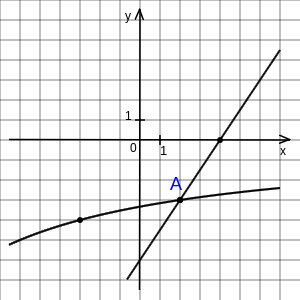
\includegraphics[width=0.4\textwidth]{images/17222136364202n0.png}
    \end{multicols}
    

\end{frame}

\begin{frame}{Задание по мотивам вариантов А. Ларина}

    \begin{multicols}{2}
        На рисунке изображён график функции вида $f (x)=|kx+b|+c$, где числа $b$, $c$ и $k$ — целые, $k \leq 0$, $b\geq0$. Найдите сумму $k+b+c$.\\

        Ответ: $-5$\\

        Решение: \\
        $f (x)=|4x-4|-5$

        
\includegraphics[width=0.4\textwidth]{images/453912618511153n0.png}
    
    \end{multicols}
\end{frame}

\begin{frame}{Этапы генерации}
    \begin{itemize}
        \item Генерация коэффициентов функций
        \item Подсчёт количества точек в узлах целочисленной решётки  \\(функция \texttt{intPoints})
        \item Отрисовка целочисленной сетки и осей координат  \\(функция \texttt{drawCoordinatePlane})
        \item Отрисовка графика  \\(функция \texttt{graph9AdrawFunction})
        \item Отображение нескольких точек в узлах решётки  \\(функция \texttt{graph9AmarkCircles})
    \end{itemize}
    
\end{frame}

\begin{frame}{Достижения}
    \begin{itemize}
        \item Полностью покрыт открытый банк заданий ФИПИ по заданию №10.
        \item Разработано 35 шаблонов
        \item В ядро добавлено несколько вспомогательных функций, которые позволят быстро разрабатывать новые шаблоны при добавлении новых прототипов в открытый банк заданий
    \end{itemize}
    
\end{frame}

\begin{frame}{Кубический сплайн}
    Кубическим сплайном функции $y = f (x)$, $x\in[a, b]$ на сетке $a=x_0<x_1<x_2< \dots <x_n=b$ назовём функцию $S(x)$, удовлетворяющую условиям:
    \begin{enumerate}
        \item На каждом отрезке $[x_{i-1},x_i]$, функция $S (x)$ является полиномом третьей степени.
        \item Функция $S (x)$, ее первая $S' (x)$ и вторая $S'' (x)$ производные непрерывны на сегменте $[a, b]$.
        \item $S (x_i)=f (x_i)=f_i, i=0,\dots,n$.
\end{enumerate}
\end{frame}  

\begin{frame}{Примеры генерации задач №7}
    
    \begin{multicols}{2}
        На рисунке изображён график $y=f' (x)$ — производной функции $f (x)$, определенной на интервале $ (-3;5)$. В какой точке отрезка $[2; 3]$ функция $f (x)$ принимает наибольшее значение?\\

        Ответ: $3$

        
\includegraphics[width=0.5\textwidth]{images/9299084059373277n0}
    \end{multicols}
          
\end{frame}

\begin{frame}{Примеры генерации задач №7}
    
    \begin{multicols}{2}
        На рисунке изображен график производной функции $f (x)$, определенной на интервале $ (-1; 8)$. Найдите количество точек, в которых касательная к графику функции $f (x)$ параллельна прямой $y=-3x+ 14{,}8 $ или совпадает с ней.\\

        Ответ: $3$

        
\includegraphics[width=0.5\textwidth]{images/776525944899729n0}
      \end{multicols}
        
   
\end{frame}

\begin{frame}{Примеры генерации задач №7}
    \begin{multicols}{2}
        На рисунке изображен график функции $y=f (x)$, определенной на~интервале $ (-6;8)$. Найдите сумму точек экстремума функции $f (x)$.\\

        Ответ: $5$

        
\includegraphics[width=0.5\textwidth]{images/020693809529216n0}
    \end{multicols}
\end{frame}

\begin{frame}{Этапы генерации}
    \begin{itemize}
        \item Генерация точек, через которые будет проходить функция
        \item Использование сторонней библиотеки \texttt{cubic-spline} для построения графика функции по точкам сплайна третьего порядка.
        \item Проверка на нахождение графика в рамках видимости %что за бред?
        \item Подсчёт и нахождение точек экстремума функции \\(функция \texttt{findExtremumOfFunction})
        \item Отрисовка графика функции
    \end{itemize}
    
\end{frame}


\begin{frame}{Достижения}
    \begin{itemize}
        \item Полностью покрыт открытый банк заданий ФИПИ по теме "Изучение графика функции и её производной".
        \item Разработано 20 шаблонов
        \item В проект добавлена сторонняя библиотека \texttt{cubic-spline}
        \item Добавлена функция для нахождения экстремумов функции
    \end{itemize}
    
\end{frame}

\begin{frame}{Список используемых источников}
    \begin{thebibliography}{10}
        \bibitem{chasdok1} Момот Е. А., Арахов Н. Д. Разработка и внедрение ПО для сбора статистики результатов подготовки к ЕГЭ по математике профильного уровня //Актуальные проблемы прикладной математики, информатики и механики. – 2021. – С. 1-2.
        \bibitem{spline}Костомаров Д. П., Фаворский А. П. Вводные лекции по численным методам.
        \bibitem{egemath}Открытый банк задач ЕГЭ по Математике.Профильный уровень. – URL:  https://prof.mathege.ru
        \bibitem{fipi}Федеральный институт педагогических измерений. – URL:  https://fipi.ru/ege/otkrytyy-bank-zadaniy-ege
        
    \end{thebibliography}
\end{frame}

\begin{frame}
    \center\Large\textcolor{NordBrightBlue}{\textbf{Спасибо за внимание}}\\
\end{frame}

\end{document}
